\graphicspath{{./figures/}}
\title{virus 2 / object formats}
\date{}
\usepackage{contour}
\begin{document}
\begin{frame}
    \titlepage
\end{frame}

{
\setbeamercolor{background canvas}{bg=blue!40!black,fg=blue!10!white}
\setbeamercolor{normal text}{bg=blue!40!black,fg=blue!10!white}
\setbeamercolor{itemize/enumerate body}{fg=white}
\setbeamercolor{itemize/enumerate subbody}{fg=white}
\setbeamercolor{titlelike}{bg=blue!40!black,fg=blue!10!white}
\begin{frame}<1|handout:1>[noframenumbering]{Changelog}
    \begin{itemize}
    \item 13 Feb 2021: add diagram showing operating of ELF LOAD program headers
    \end{itemize}
\end{frame}
}





\begin{frame}{last time}
    \begin{itemize}
    \item x86-64 encoding
        \begin{itemize}
        \item built up from 16-bit
        \item (prefix) (opcode) (mod/reg/rm) (sib) \ldots
        \item REX prefix for extra registers, 64- v 32-bit
        \item absolute versus relative address encoding
        \end{itemize}
    \item Vienna as case study
        \begin{itemize}
        \item add jmp at beginning of .COM executable files
        \item make backup copy of what replaced jmp
        \item append code to end of executable
        \item push + ret for jump back to avoid changing relative jump
        \end{itemize}
    \end{itemize}
\end{frame}

\providecommand{\myemphTwo}[1]{\myemph<2>{#1}}
\providecommand{\myemphTwoB}[1]{\myemph<2>{\textbf<2>{#1}}}
\providecommand{\myemphThree}[1]{\myemph<3>{#1}}
\providecommand{\myemphFour}[1]{\myemph<4>{#1}}
\providecommand{\myemphFive}[1]{\myemph<5>{#1}}
\providecommand{\myemphSix}[1]{\myemph<6>{#1}}
\providecommand{\myemphSeven}[1]{\myemph<7>{#1}}




\section{Case study: Vienna}


\begin{frame}<1>[label=viennaOutline]{Vienna: infection outline}
\begin{itemize}
\item Vienna \myemph{appends} code to infected application
\vspace{.5cm}
\item \myemph<2>{where does it read the code come from?}
\item \myemph<3>{how is code adjusted for new location in the binary?}
    \begin{itemize}\item what linker would do\end{itemize}
\item \myemph<4>{how does it keep files from getting infinitely long?}
\end{itemize}
\end{frame}


\subsection{Vienna relocation code}
% FIXME: need to explain why this is a problem
\againframe<3>{viennaOutline}

\subsubsection{Vienna's relocation code}

\begin{frame}[fragile,label=virusReloc2]{Vienna relocation}
\lstset{
    style=small,
    language=myasm,
    moredelim={**[is][\btHL<1|handout:0>]{@hi1@}{@endhi@}},
    moredelim={**[is][\btHL<2|handout:0>]{@hi2@}{@endhi@}},
    moredelim={**[is][\btHL<3|handout:0>]{@hi3@}{@endhi@}},
}
\begin{lstlisting}
// set virus data address:
0x700: @hi1@mov $0x8f9, %si@endhi@
       // machine code: be f9 08
       // be: opcode
       // f9 08: immediate
...
// %ax contains file length (of file to infect)
mov %ax, %cx
...
@hi3@add $0x2f9, %cx@endhi@
mov %si, %di   
sub $0x1f7, %di // %di <- 0x701
@hi2@mov %cx, (%di)@endhi@  // update mov instruction
...
\end{lstlisting}
\begin{tikzpicture}[overlay,remember picture]
\begin{visibleenv}<1>
\node[align=left,draw,very thick,fill=white] at (current page.center) {
    Vienna design: need to access global variables, etc. \\
    solution: base pointer for virus data \\
    problem: location changes depending on where virus is
};
\end{visibleenv}
\end{tikzpicture}
\end{frame}

\begin{frame}[fragile,label=virusReloc3]{Vienna relocation}
\begin{itemize}
\item edit actual code for {\tt mov}
\item why doesn't this disrupt virus execution?
    \begin{itemize}\item<2> already ran that instruction\end{itemize}
\end{itemize}
\end{frame}

\begin{frame}[fragile,label=virusReloc4]{Vienna relocation}
\lstset{
    style=smaller,
    language=myasm,
    moredelim={**[is][\btHL<2|handout:0>]{@hi2@}{@endhi@}},
    moredelim={**[is][\btHL<3|handout:0>]{@hi3@}{@endhi@}},
}
\begin{lstlisting}
0x700: mov $0x8f9, %si
...
// %ax contains file length
//     (of file to infect)
mov %ax, %cx
sub $3, %ax
// update template jmp instruction
mov %ax, @hi2@0xe(%si)@endhi@ // 0xe + %si = 0x907
...
mov $40, %ah
mov $3, %cx
mov %si, %dx  
add $0xD, @hi3@%dx@endhi@ // dx <- 0x906
int 0x21 // system call: write 3 bytes from 0x906
...
0x906: @hi2@e9 fd 05@endhi@ // jmp PC+FD 05
\end{lstlisting}
\end{frame}



\subsubsection{alternate: PIC}

\begin{frame}[fragile,label=altVirusReloc]{alternative relocation}
    \begin{itemize}
    \item could avoid having pointer to update:
    \end{itemize}
\begin{Verbatim}[fontsize=\fontsize{10}{11}\selectfont,commandchars=Q\{\}]
0000000000000000 <next-0x3>:
   0:   e8 Qtextbf{00 00}                call   3 <next>
    Qtextit{target addresses encoded relatively}
    Qtextit{pushes return address (next) onto stack}
0000000000000003 <next>:
   3:   59                      pop    %cx
    Qtextit{cx containts address of the pop instruction}
\end{Verbatim}
    \begin{itemize}
    \item why didn't Vienna do this?
    \end{itemize}
\end{frame}



\subsection{avoiding reinfection}
\againframe<4>{viennaOutline}


\begin{frame}{Vienna: avoiding reinfection}
\begin{itemize}
\item scans through active directories for executables
\item ``marks'' infected executables in \myemph{file metadata}
\begin{itemize}
    \item could have checked for virus code --- but slow
\end{itemize}
\end{itemize}
\end{frame}

\begin{frame}{DOS last-written times}
\begin{itemize}
    \item 16-bit number for date; 16-bit number for time
\end{itemize}
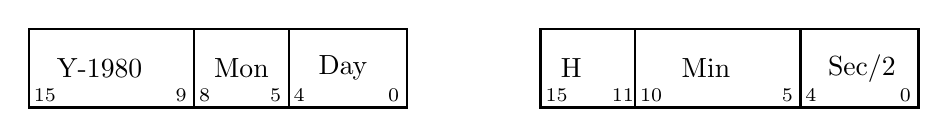
\begin{tikzpicture}
\tikzset{
    mylabel/.style={anchor=center},
    bitlabel/.style={font=\scriptsize,anchor=south west,inner sep=.5mm,text depth=.1mm},    
};
\begin{scope}[x=1.2cm]
\begin{scope}[thick]
    \draw (0, 0) rectangle (4, 1);
    \draw (0, 0) rectangle (1.75, 1);
    \node[bitlabel] at (0, 0) {15};
    \node[bitlabel] at (1.5, 0) {9};
    \draw (1.75, 0) rectangle (2.75, 1);
    \node[bitlabel] at (1.75, 0) {8};
    \node[bitlabel] at (2.5, 0) {5};
    \draw (2.75, 0) rectangle (4., 1);
    \node[bitlabel] at (2.75, 0) {4};
    \node[bitlabel] at (3.75, 0) {0};
\end{scope}
\node[mylabel] at (.75, 0.5) {Y-1980};
\node[mylabel] at (2.25, 0.5) {Mon};
\node[mylabel] at (3.325, 0.5) {Day};
\end{scope}

\begin{scope}[x=1.2cm,xshift=6.5cm]
\begin{scope}[thick]
    \draw (0, 0) rectangle (4, 1);
    \draw (0, 0) rectangle (1, 1);
    \node[bitlabel] at (0, 0) {15};
    \node[bitlabel] at (.7, 0) {11};
    \draw (1, 0) rectangle (2.75, 1);
    \node[bitlabel] at (1.0, 0) {10};
    \node[bitlabel] at (2.5, 0) {5};
    \draw (2.75, 0) rectangle (4., 1);
    \node[bitlabel] at (2.75, 0) {4};
    \node[bitlabel] at (3.75, 0) {0};
\end{scope}
\node[mylabel] at (.325, 0.5) {H};
\node[mylabel] at (1.75, 0.5) {Min};
\node[mylabel] at (3.4, 0.5) {Sec/2};
\end{scope}
\end{tikzpicture}
\begin{itemize}
    \item<2> Sec/2: 5 bits: range from 0--31
        \begin{itemize}
        \item corresponds to 0 to \textbf{62} seconds
        \end{itemize}
    \item<2> Vienna trick: set infected file times to \textbf{62} seconds
    \item<2> need to update times anyways --- hide tracks
\end{itemize}
\end{frame}



\section{reflection: how Vienna is ancient}
\begin{frame}{Vienna: on detection}
    \begin{itemize}
    \item special metadata mark could be looked for
    \item distinctive pattern, in well known place
        \begin{itemize}
        \item future assignment: pattern matching to find known malware
        \end{itemize}
    \end{itemize}
\end{frame}

\begin{frame}{Vienna: non-portability}
    \begin{itemize}
    \item \myemph<2>{relies on very simple executable formats}
        \begin{itemize}
        \item modern (read: anything after DOS) executable formats more complex/featureful
        \end{itemize}
    \item \myemph<2>{relies on self-modifying code}
        \begin{itemize}
        \item often requires extra steps on modern systems
        \end{itemize}
    \item uses metadata on filesystem
        \begin{itemize}
        \item quirk of DOS filesystem timestamp format
        \end{itemize}
    \end{itemize}
\end{frame}



% FIXME: introduce exec-format stuff, with interleave on
    % entry-points
    % how to add code

\section{executable and linking format (ELF)}
\usetikzlibrary{arrows.meta,calc,patterns,positioning}

\begin{frame}{memory v. disk}
\begin{tikzpicture}
\tikzset{
    mylabel/.style={font=\ttfamily},
    mybox/.style={draw,rectangle,minimum width=5cm,fill=white},
    myboxD/.style={draw,rectangle,minimum width=6cm,fill=white},
    myhigh/.style={draw,rectangle,line width=1mm, draw=blue!80!black,opacity=.3},
    nomem/.style={black!50,draw=black,fill=white},
}
\node[mybox,minimum height=1cm,pattern=north west lines,pattern color=black!20!white] (kernel) {Used by OS};
\node[above=.2cm of kernel] {(virtual) memory};
\node[mybox, minimum height=.5cm, below=1cm of kernel] (stack) {Stack};
\node[mybox, minimum height=.5cm, below=1cm of stack] (heap) {Heap / other dynamic};
\node[mybox, minimum height=.5cm, below=0mm of heap] (data) {Writable data};
\node[mybox, minimum height=.5cm, below=0mm of data] (sdata) {Code + Constants};
\coordinate (memBottom) at ($(sdata.south east) + (0mm, -2mm)$);
\begin{pgfonlayer}{bg}
\draw[pattern=north west lines, pattern color=black!40!white] (kernel.north west) rectangle (memBottom);
\end{pgfonlayer}

\node[myboxD,below right=4cm and 1cm of kernel,nomem] (diskHeader) {program header};
\node[myboxD,above=0cm of diskHeader] (textSeg) { {\tt .text} (code) };
\node[myboxD,above=0cm of textSeg] (rodataSeg) { {\tt .rodata} (read-only data) };
\node[myboxD,above=0cm of rodataSeg] (dataSeg) { {\tt .data} };
\node[myboxD,above=0cm of dataSeg,pattern=north west lines, pattern color=black!40] (bssSeg) { {\tt .bss} (zeroes; not stored) };
\node[above=.2cm of bssSeg] {program on disk};
\draw[very thick,-Latex] ([xshift=2mm]diskHeader.south east) -- ([xshift=2mm]bssSeg.north east) node[font=\small,midway,right,align=left] {higher \\ addresses \\ (and offsets)};


\foreach \f/\t in {textSeg/sdata,rodataSeg/sdata,dataSeg/data,bssSeg/data} {
    \draw[thick,-Latex,black] (\f.west) -- (\t.east);
}
\end{tikzpicture}

% FIXME: add animation: binary file format
\end{frame}

\begin{frame}{ELF (executable and linking format)}
\begin{itemize}
\item Linux {\small (and some others)} executable/object file format
\end{itemize}
\begin{tikzpicture}
\tikzset{
    mybox/.style={draw,rectangle,minimum width=10cm,fill=white},
}
\node[mybox] (header) {
    \textbf{header}: machine type, file type, etc.
};
\node[mybox,below=0mm of header,align=center] (pHeader) {
    \textbf{program header}: ``\myemph{segments}'' to load \\
        (also, some other information)
};
\node[mybox,below=0mm of pHeader,align=center] (seg1) {
    \textbf{segment 1 data}
};
\node[mybox,below=0mm of seg1,align=center] (seg2) {
    \textbf{segment 2 data}
};
\node[mybox,below=3mm of seg2,align=center] (seg2) {
    \textbf{section header}:  \\ list of ``\myemph{sections}''(mostly for linker)
};
\end{tikzpicture}
\end{frame}

\begin{frame}{segments versus sections?}
\begin{itemize}
    \item note: ELF terminology; may not be true elsewhere!
    \item sections --- \myemph{object files} {\small (and usually executables)}, used by \myemph{linker}
        \begin{itemize}
        \item have information on intended purpose
        \item linkers combine these to create executables
        \item linkers might omit unneeded sections
        \end{itemize}
    \item segments --- executables, used to actually load program
        \begin{itemize}
        \item program loader is \myemph{dumb} --- doesn't know what segments are for
        \end{itemize}
\end{itemize}
\end{frame}




\subsection{ELF sections}
\usetikzlibrary{calc}

\begin{frame}[fragile,label=sectHeader]{section headers}
\vspace{-.25cm}
\begin{Verbatim}[fontsize=\tiny]
Sections:
Idx Name          Size      VMA               LMA               File off  Algn
  0 .note.ABI-tag 00000020  0000000000400190  0000000000400190  00000190  2**2
                  CONTENTS, ALLOC, LOAD, READONLY, DATA
  1 .note.gnu.build-id 00000024  00000000004001b0  00000000004001b0  000001b0  2**2
                  CONTENTS, ALLOC, LOAD, READONLY, DATA
  2 .rela.plt     00000210  00000000004001d8  00000000004001d8  000001d8  2**3
                  CONTENTS, ALLOC, LOAD, READONLY, DATA
  3 .init         0000001a  00000000004003e8  00000000004003e8  000003e8  2**2
                  CONTENTS, ALLOC, LOAD, READONLY, CODE
  4 .plt          00000160  0000000000400410  0000000000400410  00000410  2**4
                  CONTENTS, ALLOC, LOAD, READONLY, CODE
  5 .text         0017ff1d  0000000000400570  0000000000400570  00000570  2**4
                  CONTENTS, ALLOC, LOAD, READONLY, CODE
  6 __libc_freeres_fn 00002032  0000000000580490  0000000000580490  00180490  2**4
                  CONTENTS, ALLOC, LOAD, READONLY, CODE
  7 __libc_thread_freeres_fn 0000021b  00000000005824d0  00000000005824d0  001824d0  2**4
                  CONTENTS, ALLOC, LOAD, READONLY, CODE
  8 .fini         00000009  00000000005826ec  00000000005826ec  001826ec  2**2
                  CONTENTS, ALLOC, LOAD, READONLY, CODE
  9 .rodata       00044ac8  0000000000582700  0000000000582700  00182700  2**6
                  CONTENTS, ALLOC, LOAD, READONLY, DATA
 10 __libc_subfreeres 000000c0  00000000005c71c8  00000000005c71c8  001c71c8  2**3
                  CONTENTS, ALLOC, LOAD, READONLY, DATA
 11 .stapsdt.base 00000001  00000000005c7288  00000000005c7288  001c7288  2**0
                  CONTENTS, ALLOC, LOAD, READONLY, DATA
 12 __libc_atexit 00000008  00000000005c7290  00000000005c7290  001c7290  2**3
                  CONTENTS, ALLOC, LOAD, READONLY, DATA
 13 __libc_thread_subfreeres 00000018  00000000005c7298  00000000005c7298  001c7298  2**3
                  CONTENTS, ALLOC, LOAD, READONLY, DATA
 14 .eh_frame     000141dc  00000000005c72b0  00000000005c72b0  001c72b0  2**3
                  CONTENTS, ALLOC, LOAD, READONLY, DATA
 15 .gcc_except_table 0000020b  00000000005db48c  00000000005db48c  001db48c  2**0
                  CONTENTS, ALLOC, LOAD, READONLY, DATA
 16 .tdata        00000030  00000000007dbea8  00000000007dbea8  001dbea8  2**3
                  CONTENTS, ALLOC, LOAD, DATA, THREAD_LOCAL
 17 .tbss         0000004a  00000000007dbed8  00000000007dbed8  001dbed8  2**3
                  ALLOC, THREAD_LOCAL
 18 .init_array   00000010  00000000007dbed8  00000000007dbed8  001dbed8  2**3
                  CONTENTS, ALLOC, LOAD, DATA
 19 .fini_array   00000010  00000000007dbee8  00000000007dbee8  001dbee8  2**3
                  CONTENTS, ALLOC, LOAD, DATA
 20 .jcr          00000008  00000000007dbef8  00000000007dbef8  001dbef8  2**3
                  CONTENTS, ALLOC, LOAD, DATA
 21 .data.rel.ro  000000e8  00000000007dbf00  00000000007dbf00  001dbf00  2**6
                  CONTENTS, ALLOC, LOAD, DATA
 22 .got          00000010  00000000007dbfe8  00000000007dbfe8  001dbfe8  2**3
                  CONTENTS, ALLOC, LOAD, DATA
 23 .got.plt      000000c8  00000000007dc000  00000000007dc000  001dc000  2**3
                  CONTENTS, ALLOC, LOAD, DATA
 24 .data         00001f96  00000000007dc100  00000000007dc100  001dc100  2**6
                  CONTENTS, ALLOC, LOAD, DATA
 25 .bss          00005a90  00000000007de0c0  00000000007de0c0  001de096  2**6
                  ALLOC
 26 __libc_freeres_ptrs 00000070  00000000007e3b50  00000000007e3b50  001de096  2**3
                  ALLOC
 27 .note.stapsdt 0000100c  0000000000000000  0000000000000000  001de098  2**2
                  CONTENTS, READONLY
 28 .gnu_debuglink 00000034  0000000000000000  0000000000000000  001df0a4  2**0
                  CONTENTS, READONLY
\end{Verbatim}
\end{frame}

\begin{frame}{sections}
\begin{itemize}
\item tons of ``sections''
\item not actually needed/used to run program
\item size, file offset, flags (code/data/etc.)
    \begin{itemize}
    \item location in executable \textit{and} in memory
    \end{itemize}
\item some sections aren't stored (no ``CONTENTS'' flag) 
    \begin{itemize}
    \item just all zeroes
    \end{itemize}
\end{itemize}
\end{frame}

\begin{frame}{selected sections}
\begin{tabular}{rl}
    {\tt .text} & program code \\
    {\tt .bss} & initially zero data {\scriptsize (block started by symbol)} \\
    {\tt .data} & other writeable data  \\
    {\tt .rodata} & read-only data \\
    {\tt .init}/{\tt .fini} & global constructors/destructors \\
    {\tt .got}/{\tt .plt} & dynamic linking related \\
    {\tt .eh\_frame} & try/catch related \\
\end{tabular}
\imagecredit{based on \url{http://people.redhat.com/mpolacek/src/devconf2012.pdf}}
\end{frame}




\subsection{program headers: example static ELF binary}
\providecommand{\myemphTwo}[1]{\myemph<2>{#1}}
\providecommand{\myemphTwoB}[1]{\myemph<2>{\textbf<2>{#1}}}
\providecommand{\myemphThree}[1]{\myemph<3>{#1}}
\providecommand{\myemphFour}[1]{\myemph<4>{#1}}
\providecommand{\myemphFive}[1]{\myemph<5>{#1}}
\providecommand{\myemphSix}[1]{\myemph<6>{#1}}
\providecommand{\myemphSeven}[1]{\myemph<7>{#1}}

\begin{frame}[fragile,label=elfExOver1]{ELF example}
    \begin{itemize}
    \item {\tt objdump -x /bin/busybox} (on my laptop)
    \item {\tt -x}: output all headers
    \end{itemize}
\begin{Verbatim}[commandchars=\\\{\},fontsize=\small]
/bin/busybox:     file format \myemphTwo{elf64-x86-64}
/bin/busybox
architecture: i386:x86-64, flags 0x00000102:
EXEC_P, D_PAGED
start address \myemphThree{0x0000000000402170}

Program Header:
[...]

Sections:
[...]
\end{Verbatim}
\end{frame}

\begin{frame}[fragile,label=elfExOver2]{a program header (1)}
\begin{Verbatim}[commandchars=\\\{\},fontsize=\fontsize{9}{10}\selectfont]
Program Header:
[...]
LOAD off    0x0001000 vaddr 0x0401000 paddr 0x0401000 align 2**12
     filesz \myemphTwo{0x01b04ed} memsz 0x01b04ed flags \myemphThree{r-x}
[...]
LOAD off    0x0207950 vaddr 0x0608950 paddr 0x0608950 align 2**12
     filesz \myemphFour{0x0008f40} memsz \myemphFour{0x000c718} flags rw-

\end{Verbatim}
\begin{itemize}
\item load {\tt \myemph<2>{0x1bd04ed}} bytes:
        \begin{itemize}
        \item from {\tt 0x1000} bytes into the file 
        \item to memory at {\tt 0x401000} \\
        \item \myemph<3>{readable and executable}
        \end{itemize}
\item load {\tt 0x8f40} bytes:
        \begin{itemize}
        \item from {\tt 0x207950} bytes into the file 
        \item to memory at {\tt 0x608950} 
        \item \myemph<4>{plus ({\tt 0xc718}--{\tt 0x8f40}) bytes of zeroes}
        \item readable and writable
        \end{itemize}
\end{itemize}
\end{frame}

\begin{frame}[fragile,label=elfExOver3]{a program header (2)}
\begin{Verbatim}[commandchars=\\\{\},fontsize=\fontsize{9}{10}\selectfont]
Program Header:
[...]
    NOTE off    0x0000290 vaddr 0x0400290 paddr 0x0400290 align 2**2
         filesz 0x0000044 memsz 0x0000044 flags r--
     TLS off    0x0207950 vaddr 0x0608950 paddr 0x0608950 align 2**3
         filesz 0x0000030 memsz 0x0000092 flags r--
0x6474e553 off  0x0000270 vaddr 0x0400270 paddr 0x0400270 align 2**3
         filesz 0x0000020 memsz 0x0000020 flags r--
   STACK off    0x0000000 vaddr 0x0000000 paddr 0x0000000 align 2**4
         filesz 0x0000000 memsz 0x0000000 flags rw-
   RELRO off    0x0207950 vaddr 0x0608950 paddr 0x0608950 align 2**0
         filesz 0x00066b0 memsz 0x00066b0 flags r--
[...]
\end{Verbatim}
\begin{itemize}
\item NOTE --- comment
\item TLS --- thread-local storage region (used via {\tt \%fs})
\item 0x6474e553 --- `GNU\_PROPERTY' --- adtl linker/loader info
\item STACK --- indicates stack is read/write
\item RELRO --- make this read-only after runtime linking
\end{itemize}
\end{frame}




\subseciton{diagram: ELF loading}
\usetikzlibrary{arrows.meta,decorations.pathmorphing,patterns}

\begin{frame}<2->{ELF LOAD}
\begin{tikzpicture}
\begin{pgfonlayer}{fg}
    \draw[very thick] (0, 0) rectangle (4, 6);
\node[font=\huge,black!25,align=center] at (2, 3) {
    program \\ on\\ disk
};
\end{pgfonlayer}
\coordinate (header tl) at (4, 0.5);
\coordinate (header br) at (0, 0);
\coordinate (load off) at (0, 1);
\coordinate (load end) at (0, 2.54);
\draw[thick,Latex-,font=\small] (0, 0) -- ++(-.5, 0) node[left,align=right] {off {\tt 0}\\ (start)};

\begin{scope}[xshift=6cm]
    \begin{pgfonlayer}{fg}
        \draw[very thick] (0, 7) -- (0, 0) -- (4, 0) -- (4, 7);
        \draw[overlay,very thick,decorate,decoration={zigzag,segment length=2.5mm}] (0, 7) -- (4, 7);
    \node[font=\huge,black!25,align=center] at (2, 3) {
        program \\ in\\ memory
    };
    \end{pgfonlayer}
    \coordinate (vaddr off) at (4, 4);
    \coordinate (vaddr end copy) at (4, 5.54);
    \coordinate (vaddr end all) at (4, 6.64);
\draw[thick,Latex-,font=\small] (4, 0) -- ++(.5, 0) node[right,align=left] {addr {\tt 0}};
\end{scope}
\begin{visibleenv}<2->
    \fill[blue!30] (header tl) rectangle (header br);
    \node[align=left,font=\small\tt,anchor=north west,draw] (load) at (1, -.25) {
        LOAD off {\color{green!50!black}0x1000} vaddr {\color{violet!70}0x4000} \ldots \\
        \hspace{1cm} filesz 0x1544 memsz 0x2644 \ldots
    };
    \draw[dotted,thick] ([yshift=-1mm]header tl -| header br) -- (load.north west);
    \draw[dotted,thick] ([xshift=3cm,yshift=-1mm]header tl -| header br) -- (load.north east);
\end{visibleenv}
\begin{visibleenv}<3->
    \draw[very thick,Latex-] (load off) -- ++(-.5cm,0) node[left,font=\small] {{\color{green!50!black}\tt 0x1000}};
    \draw[very thick,Latex-] (vaddr off) -- ++ (.5cm, 0) node[right,font=\small] {{\color{violet!70}\tt 0x4000}};
    \draw[thick,Latex-Latex] ([xshift=-.15cm]load off) -- ([xshift=-.15cm]load end)
        node[midway,font=\small,left] {\tt 0x1544};
    \draw[thick,Latex-Latex] ([xshift=.15cm]vaddr off) -- ([xshift=.15cm]vaddr end copy)
        node[midway,font=\small,right] {\tt 0x1544};
    \draw[thick,Latex-Latex] ([xshift=-4.15cm]vaddr off) -- ([xshift=-4.15cm]vaddr end all)
        node[midway,font=\small,left] {\tt 0x2644};
    \fill[red!20] (load off) rectangle ([xshift=4cm]load end);
    \fill[red!20] (vaddr off) rectangle ([xshift=-4cm]vaddr end copy);
    \fill[pattern=north west lines] (vaddr end copy) rectangle ([xshift=-4cm]vaddr end all);
\end{visibleenv}
\end{tikzpicture}
\end{frame}


% FIXME: exercise: on elf
\subsection{exercise}
\begin{frame}[fragile,label=elfStaticEx]{exercise}
\begin{Verbatim}[commandchars=\\\{\},fontsize=\small]
LOAD off    0x0000000 vaddr 0x00400000 paddr 0x00400000 align 2**12
     filesz 0x0000518 memsz 0x00000518 flags r--
LOAD off    0x0001000 vaddr 0x00401000 paddr 0x00401000 align 2**12
     filesz 0x009352d memsz 0x0009352d flags r-x
LOAD off    0x0095000 vaddr 0x00495000 paddr 0x00495000 align 2**12
     filesz 0x00265e5 memsz 0x000265e5 flags r--
LOAD off    0x00bc0c0 vaddr 0x004bd0c0 paddr 0x004bd0c0 align 2**12
     filesz 0x0006170 memsz 0x000078c0 flags rw-
\end{Verbatim}
\begin{itemize}
\item Q1: about how large is this executable on disk?
\item Q2: this executable contains a global array declared like \\\texttt{int array[SIZE] = {...};} \\
        what is the largest plausible value for SIZE based on the header?
\end{itemize}
\end{frame}


\subsection{aside on virtual memory}

\providecommand{\myemphTwo}[1]{\myemph<2>{#1}}
\providecommand{\myemphTwoB}[1]{\myemph<2>{\textbf<2>{#1}}}
\providecommand{\myemphThree}[1]{\myemph<3>{#1}}
\providecommand{\myemphFour}[1]{\myemph<4>{#1}}
\providecommand{\myemphFive}[1]{\myemph<5>{#1}}
\providecommand{\myemphSix}[1]{\myemph<6>{#1}}
\providecommand{\myemphSeven}[1]{\myemph<7>{#1}}




\begin{frame}{ELF loading: pages}
\begin{itemize}
    \item Linux, most other OSes manage memory/files in \textit{pages}
        \begin{itemize}
        \item hardware feature: virtual memory
        \item on x86-64: typically 4096 bytes
        \end{itemize}
    \item changes how LOADs work:
        \begin{itemize}
        \item offset must be rounded to multiple of page size
        \item size loaded rounded up to whole number of pages
        \end{itemize}
\end{itemize}
\end{frame}

\begin{frame}[fragile,label=ElfLoadPg]{ELF loading: pages example}
program header:
\begin{Verbatim}[fontsize=\small,commandchars=\\\{\}]
LOAD off    0x0000000 vaddr 0x00400000 paddr 0x00400000 align 2**12
     filesz 0x0000\myemphTwo{518} memsz 0x00000518 flags r--
LOAD off    0x0001000 vaddr 0x00401000 paddr 0x00401000 align 2**12
     filesz 0x00\myemphThree{9352d} memsz 0x0009352d flags r-x
LOAD off    0x0095000 vaddr 0x00495000 paddr 0x00495000 align 2**12
     filesz 0x00\myemphThree{265e5} memsz 0x000265e5 flags r--
LOAD off    0x00bc0c0 vaddr 0x004bd0c0 paddr 0x004bd0c0 align 2**12
     filesz 0x000\myemphFour{6170} memsz 0x000078c0 flags rw-
\end{Verbatim}
\hrule
actually loaded (via Linux \texttt{/proc/PID/maps}):
\begin{Verbatim}[fontsize=\small,commandchars=\\\{\}]
memory address       size        r/w? file offset
~~~~~~~~~~~~~~~~~ (~~~~~~~~)     ~~~~ ~~~~~~~~ 
00400000-00401000 (  \myemphTwo{0x1000})     r--p 00000000
00401000-00495000 ( \myemphThree{0x94000})     r-xp 00001000
00495000-004bc000 ( \myemphThree{0x27000})     r--p 00095000
004bd000-004c0000 (  \myemphFour{0x3000})     r--p 000bc000
004c0000-004c4000 (  \myemphFour{0x4000})     rw-p 000bf000
\end{Verbatim}
\end{frame}


\subsection{preview: dynamic linking/PIE}
\begin{frame}{preview: dynamic linking}
    \begin{itemize}
    \item shown so far:
    \item statically linked executables
        \begin{itemize}
        \item include all library code (instead of loading it from other files)
        \end{itemize}
    \item whose code is loaded at fixed address
        \begin{itemize}
        \item instead of that address being changeable
        \end{itemize}
    \vspace{.5cm}
    \item most common today: \\dynamically-linked, position-independent executables
    \end{itemize}
\end{frame}



\section{viruses: where to put code}


\begin{frame}{where to put code}
    \begin{itemize}
    \item viruses insert code in other programs
    \item Vienna's choice: end of executables
    \item search for \texttt{.COM} executables on system
    \vspace{.5cm}
    \item considerations for other options:
    \item spreading: identifying useful files to infect
        \begin{itemize}
        \item will be copied elsewhere?
        \item will be run?
        \end{itemize}
    \item stealth: avoiding detection
        \begin{itemize}
        \item Vienna: file size changes --- easy to find?
        \item Vienna: weird modification time --- easy to find?
        \end{itemize}
    \end{itemize}
\end{frame}

\begin{frame}<1>[label=whereCode]{where to put code: options}
    \begin{itemize}
    \item one \textit{or more} of:
    \item \myemph<2>{replacing executable code}
    \item \myemph<3>{after executable code (Vienna)}
    \item \myemph<4>{in unused executable code}
    \item \myemph<5>{inside OS code}
    \item \myemph<6>{in memory}
    \item \myemph<7>{replace existing code}
    \end{itemize}
\end{frame}



\subsection{replacing executables?}

\againframe<2>{whereCode}

\usetikzlibrary{arrows.meta}

\begin{frame}{replace executable}
    \begin{tikzpicture}
    \draw[thick] (0, 0) rectangle (4, -6) node[midway,align=center] {original\\executable};
    \draw[line width=2mm,-Latex,black!60] (4.1, -3) -- (6.9, -.5);
    \begin{scope}[xshift=7cm]
    \draw[thick,fill=red!20] (0, 0) rectangle (4, -1) node[midway,align=center] {virus code};
    \end{scope}
    \end{tikzpicture}
\end{frame}

\begin{frame}{replace executable?}
    \begin{itemize}
    \item seems silly --- not stealthy!
    \item has appeared in the wild --- ILOVEYOU
    \item 2000 ILOVEYOU Worm
        \begin{itemize}
        \item written in Visual Basic (!)
        \item spread via email
        \item replaced lots of files with copies of itself
        \end{itemize}
    \item huge impact --- because destroying data to copy itself
    \end{itemize}
\end{frame}

\begin{frame}{replace executable --- subtle}
    \begin{tikzpicture}
    \draw[thick] (0, 0) rectangle (4, -6) node[midway,align=center] {original\\executable};
    \draw[line width=2mm,-Latex,black!60] (4.1, -3) -- (6.9, -.5);
    \begin{scope}[xshift=7cm]
    \draw[thick,fill=red!20] (0, 0) rectangle (4, -1) node[midway,align=center] {virus code};
    \draw[thick,fill=yellow!20] (0, -1) rectangle (4, -1.5) node[midway,align=center,font=\scriptsize] {
        run original from tempfile
    };
    \draw[thick] (0, -1.5) rectangle (4, -7.2) node[midway,align=center] {original\\executable};
    \end{scope}
    \end{tikzpicture}
\end{frame}




\subsection{appending/compressing}

% FIXME: good place for aside on modern executable formats

\againframe<3>{whereCode}

\usetikzlibrary{arrows.meta,patterns}
\begin{frame}{appending}
    \pdftooltip{
    \begin{tikzpicture}
    \draw[thick] (0, 0) rectangle (4, -5) node[midway,align=center] {original\\executable};
    \draw[line width=2mm,-Latex,black!60] (4.1, -3) -- (6.9, -3);
    \begin{scope}[xshift=7cm]
    \draw[thick] (0, 0) rectangle (4, -5) node[midway,align=center] {original\\executable};
    \draw[fill=red!20,thick] (0, -5) rectangle (4, -6)
        node[midway,align=center] {virus code};
    \draw[fill=red!20,thick] (0.5, -1) rectangle (1, -1.5);
    \node[anchor=west,red!50!black] at (1.25, -1.25) {jmp to virus};
    \draw[thick,Latex-] (1, -1.25) -- (1.4, -1.25);
    \end{scope}
    \end{tikzpicture}
    }{executable transformed by replacing some of the original code with jmp + appending virus}
\end{frame}

\begin{frame}{appending and executable formats}
    \begin{itemize}
    \item COM files are very simple --- no metadata
    \item modern executable formats have length information to update:
    \vspace{.5cm}
    \item option 1: add segment (ELF LOAD) to program header
        \begin{itemize}
        \item (often a little extra space after program header, due to page-alignment)
        \end{itemize}
    \item option 2: update last segment of program header
        \begin{itemize}
        \item change its size
        \item make it executable if it isn't (and often not --- often data)
        \end{itemize}
    \end{itemize}
\end{frame}






\section{backup slides}
\begin{frame}{backup slides}
\end{frame}

\subsection{Vienna intro}

\begin{frame}{Case Study: Vienna Virus}
\begin{itemize}
    \item Vienna: virus from the 1980s
    \item This version: published in Ralf Burger, ``Computer Viruses: a high-tech disease'' (1988)
    \item targetted COM-format executables on DOS
\end{itemize}
\end{frame}




\subsection{aside: COM files}


\begin{frame}{Diversion: .COM files}
    \begin{itemize}
    \item .COM is a \myemph{very simple} executable format
    \item no header, no segments, no sections
    \item file contents loaded at fixed address {\tt 0x0100}
    \item execution starts at {\tt 0x0100}
    \item everything is read/write/execute (no virtual memory)
    \end{itemize}
\end{frame}




\subsection{entry/exit}

\usetikzlibrary{calc}

\begin{frame}[fragile,label=vienna]{Vienna: infection}
\lstset{
    language=myasm,
    style=smaller,
    moredelim={**[is][\btHL<2>]{~hi2~}{~endhi2~}},
}
\begin{tikzpicture}
\tikzset{programBox/.style={draw,thick},every label/.style={inner sep=1mm,outer sep=0mm}}
\node[programBox,minimum height=3cm,label={north:uninfected},anchor=north west] (uninfect) at (0,0) {
\begin{lstlisting}
0x0100:
    ~hi2~mov $0x4f28, %cx~endhi2~
    /* b9 28 4f */
0x0103:
    mov $0x9e4e, %si
    /* be 4e 9e */
    mov %si, %di
    push %ds
    /* more normal
       program
       code */
....
0x0700: /* end */

\end{lstlisting}
};
\node[overlay,programBox,anchor=north west,label={[overlay]north:infected}] at ([yshift=.5cm,xshift=1cm]uninfect.north east) {
\begin{lstlisting}
0x0100: jmp 0x0700
0x0103: mov $0x9e4e, %si
...
0x0700:
    push %cx
    ... // %si <- 0x903
    mov $0x100, %di
    mov $3, %cx
    rep movsb
    ...
    mov $0x0100, %di
    push %di
    xor %di, %di
    ret
...
0x0903:
    ~hi2~.bytes 0xb9 0x28 0x4f~endhi2~
...
\end{lstlisting}
};
\end{tikzpicture}
\end{frame}

\begin{frame}[fragile,label=viennaFixup]{Vienna: ``fixup''}
\lstset{
    language=myasm,
    style=small,
    moredelim={**[is][\btHL<2>]{~hi2~}{~endhi2~}},
    moredelim={**[is][\btHL<3>]{~hi3~}{~endhi3~}},
}
\begin{lstlisting}
0x0700:
    push %cx // initial value of %cx matters??
    mov ~hi3~$0x8fd~endhi3~, %si // %si <- beginning of data
    mov %si, %dx // save %si
        // movsb uses %si, so
        // can't use another register
    add $0xa, %si // offset of saved code in data
    mov $0x100, %di // target address
    mov $3, %cx // bytes changed
    /* copy %cx bytes from (%si) to (%di) */
    rep movsb 
    ...
...
// saved copy of original application code
0x903: ~hi2~.byte 0xb9 .byte 0x28 .byte 0x4f~endhi2~
\end{lstlisting}
\end{frame}

\begin{frame}[fragile,label=viennaReturn]{Vienna: return}
\lstset{language=myasm,style=small}
\begin{lstlisting}
0x08e7:
    pop %cx // restore initial value of %cx, %sp
    xor %ax, %ax // %ax <- 0
    xor %bx, %bx
    xor %dx, %dx
    xor %si, %si
    // push 0x0100
    mov $0x0100, %di
    push %di 
    xor %di, %di // %di <- 0
    // pop 0x0100 from stack
    // jmp to 0x0100
    ret 
\end{lstlisting}
\begin{itemize}
\item<1> question: why not just jmp 0x0100 ?
\end{itemize}
\end{frame}




\subsection{writing your own code?}

\againframe<2>{viennaOutline}
\subsubsection{aside: quines}


\begin{frame}{quines}
\begin{itemize}
    \item exercise: write a C program that outputs its source code
        \begin{itemize}
        \item (pseudo-code only okay)
        \end{itemize}
    \item possible in any {\small (Turing-complete)} programming language
    \item called a ``quine''
\end{itemize}
\end{frame}

\begin{frame}[fragile,label=quineClever]{clever quine solution}
\lstset{language=C,style=small,
    moredelim={**[is][\btHL<2|handout:0>]{@hi2@}{@endhi@}},
    moredelim={**[is][\btHL<3|handout:0>]{@hi3@}{@endhi@}},
    showstringspaces=false,
}
\begin{lstlisting}
#include <stdio.h>
char*x="int main(){
       `\btHL<2>{printf(p,10,34,x,34,10,34,p,34,10,x,10);}`
       }";
@hi3@char*p@endhi@="#include <stdio.h>%c
    char*x=%c%s%c;%cchar*p=%c%s%c;
    %c%s%c";
int main(){
    @hi2@printf(p,10,34,x,34,10,34,p,34,10,x,10);@endhi@
}
\end{lstlisting}
\begin{itemize}
\item some line wrapping for readability --- shouldn't be in actual quine
\end{itemize}
\begin{tikzpicture}[overlay,remember picture]
    \begin{visibleenv}<2|handout:0>
        \node[fill=white,draw,thick,align=left] at (current page.center) {
            {\tt printf} to fill template: \\
            {\tt 10} = newline; {\tt 34} = double-quote; \\
            {\tt x}, {\tt p} = template/constant strings
        };
    \end{visibleenv}
    \begin{visibleenv}<3|handout:0>
        \node[fill=white,draw,thick,align=left] at ([yshift=1cm]current page.center) {
            template filled by printf
        };
    \end{visibleenv}
\end{tikzpicture}
\end{frame}

\begin{frame}[fragile,label=quineDumb]{dumb quine solution}
\begin{lstlisting}[language=C,style=small]
#include <stdio.h>
int main(void) {
    char buffer[1024];
    FILE *f = fopen("quine.c", "r");
    size_t bytes = fread(buffer, 1,
                         sizeof(buffer), f);
    fwrite(buffer, 1, bytes, stdout);
    return 0;
}
\end{lstlisting}
\begin{itemize}
\item a lot more straightforward!
\item but ``cheating''
\end{itemize}
\end{frame}




\subsubsection{Vienna replication code}


\begin{frame}[fragile,label=virusWriting]{Vienna copying}
\lstset{
    style=small,
    language=myasm,
    moredelim={**[is][\btHL<2|handout:0>]{@hi2@}{@endhi@}},
}
\begin{lstlisting}
@hi2@mov $0x8f9, %si@endhi@ // %si = beginning of virus data
...
mov $0x288, %cx // length of virus
mov $0x40, %ah  // system call # for write
mov %si, %dx
sub $0x1f9, %dx // %dx = beginning of virus code
int 0x21 // make write system call
\end{lstlisting}
\end{frame}






\end{document}
